\section{Datasets for Sound Event Classification}

\subsection{Acoustic Road Roughness Classification}
The dataset built for this work is done with a multi-channel microphone arrangement, with the prospect of conducting different assessments at once or to exploit microphone diversity to improve the classification. More specifically, two microphones have been placed close to the rear wheels, one in front of the front left wheel, one inside the engine compartment and two inside the cockpit, close to the driver head and close to the right passenger head. The rear wheel microphones have been placed off-axis, in order to avoid dirt from the wheel and protected by the wheelhouse to reduce the effect of wind. Figure \ref{fig:car-mic} shows the positioning of all microphones. External microphones are \textit{PCB Piezotronics} model 130A24. These are IP55 microphones and they have been protected with a melamine resin foam for sound absorption to reduce the effect of wind. The internal microphones are \textit{PCB Piezotronics} model 378C20. The front-right wheel has been excluded from recordings after first informal evaluations because it picked a large amount of engine noise with respect to the other microphones. The rear-right microphone, vice versa, was found to be the best choice because the noise from the engine was the lowest and it has been used for this first evaluation. The engine compartment microphone has been used to record the engine conditions for future use. In \figref{fig:car-rr-and-fl} are shown the images of the microphones installation. 

\begin{figure}[ht]
	\centering
	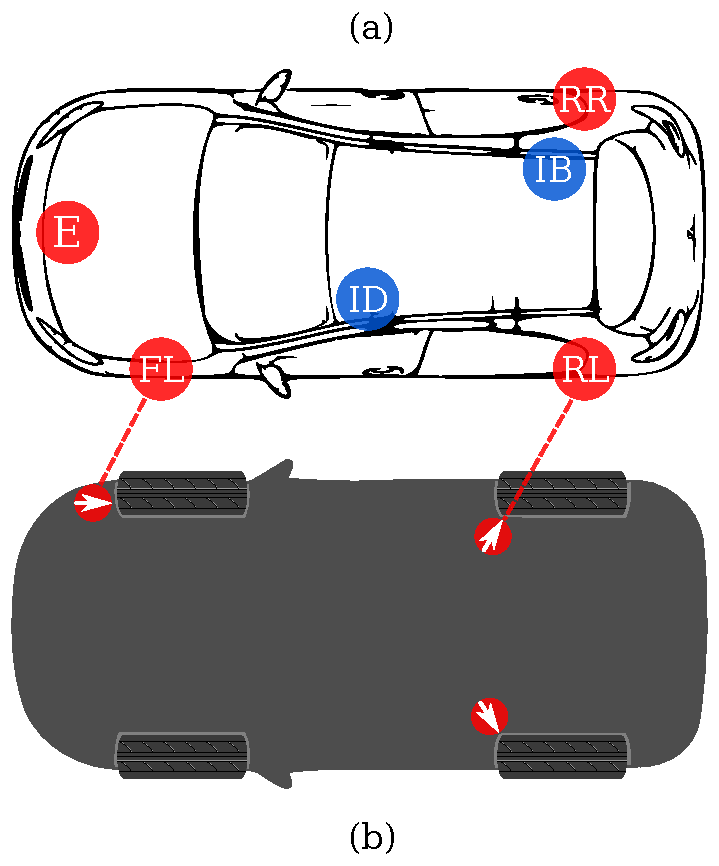
\includegraphics[width=0.5\textwidth]{img/car-mic}
	\caption[Position of the microphones in the car used to record the dataset]{Positioning of the microphones in the car used to record the dataset, top view (a) and bottom view (b). The microphones are placed in the engine compartment (E), close to the front-left, rear-left and rear-right tyres (FL, RL, RR), and inside the car close to the driver or in the back seat (ID, IB). The last two microphones are \textit{PCB Piezotronics} model 378C20 type microphones, while all the others are IP55 \textit{PCB Piezotronics} model 130A24 microphones. The microphones are omnidirectional, however the arrows in (b) show how the capsule was positioned to minimize wind effect. The rear microphones are protected in the wheelhouse.}
	\label{fig:car-mic}
\end{figure}

\begin{figure}[t]
	\centering
	\begin{subfigure}[b]{0.48\textwidth}
		\includegraphics[width=\textwidth]{img/Rear-Right.jpg}
		\subcaption{Rear right tyre microphone.}
	\end{subfigure}
	\hfil
	\begin{subfigure}[b]{0.48\textwidth}
		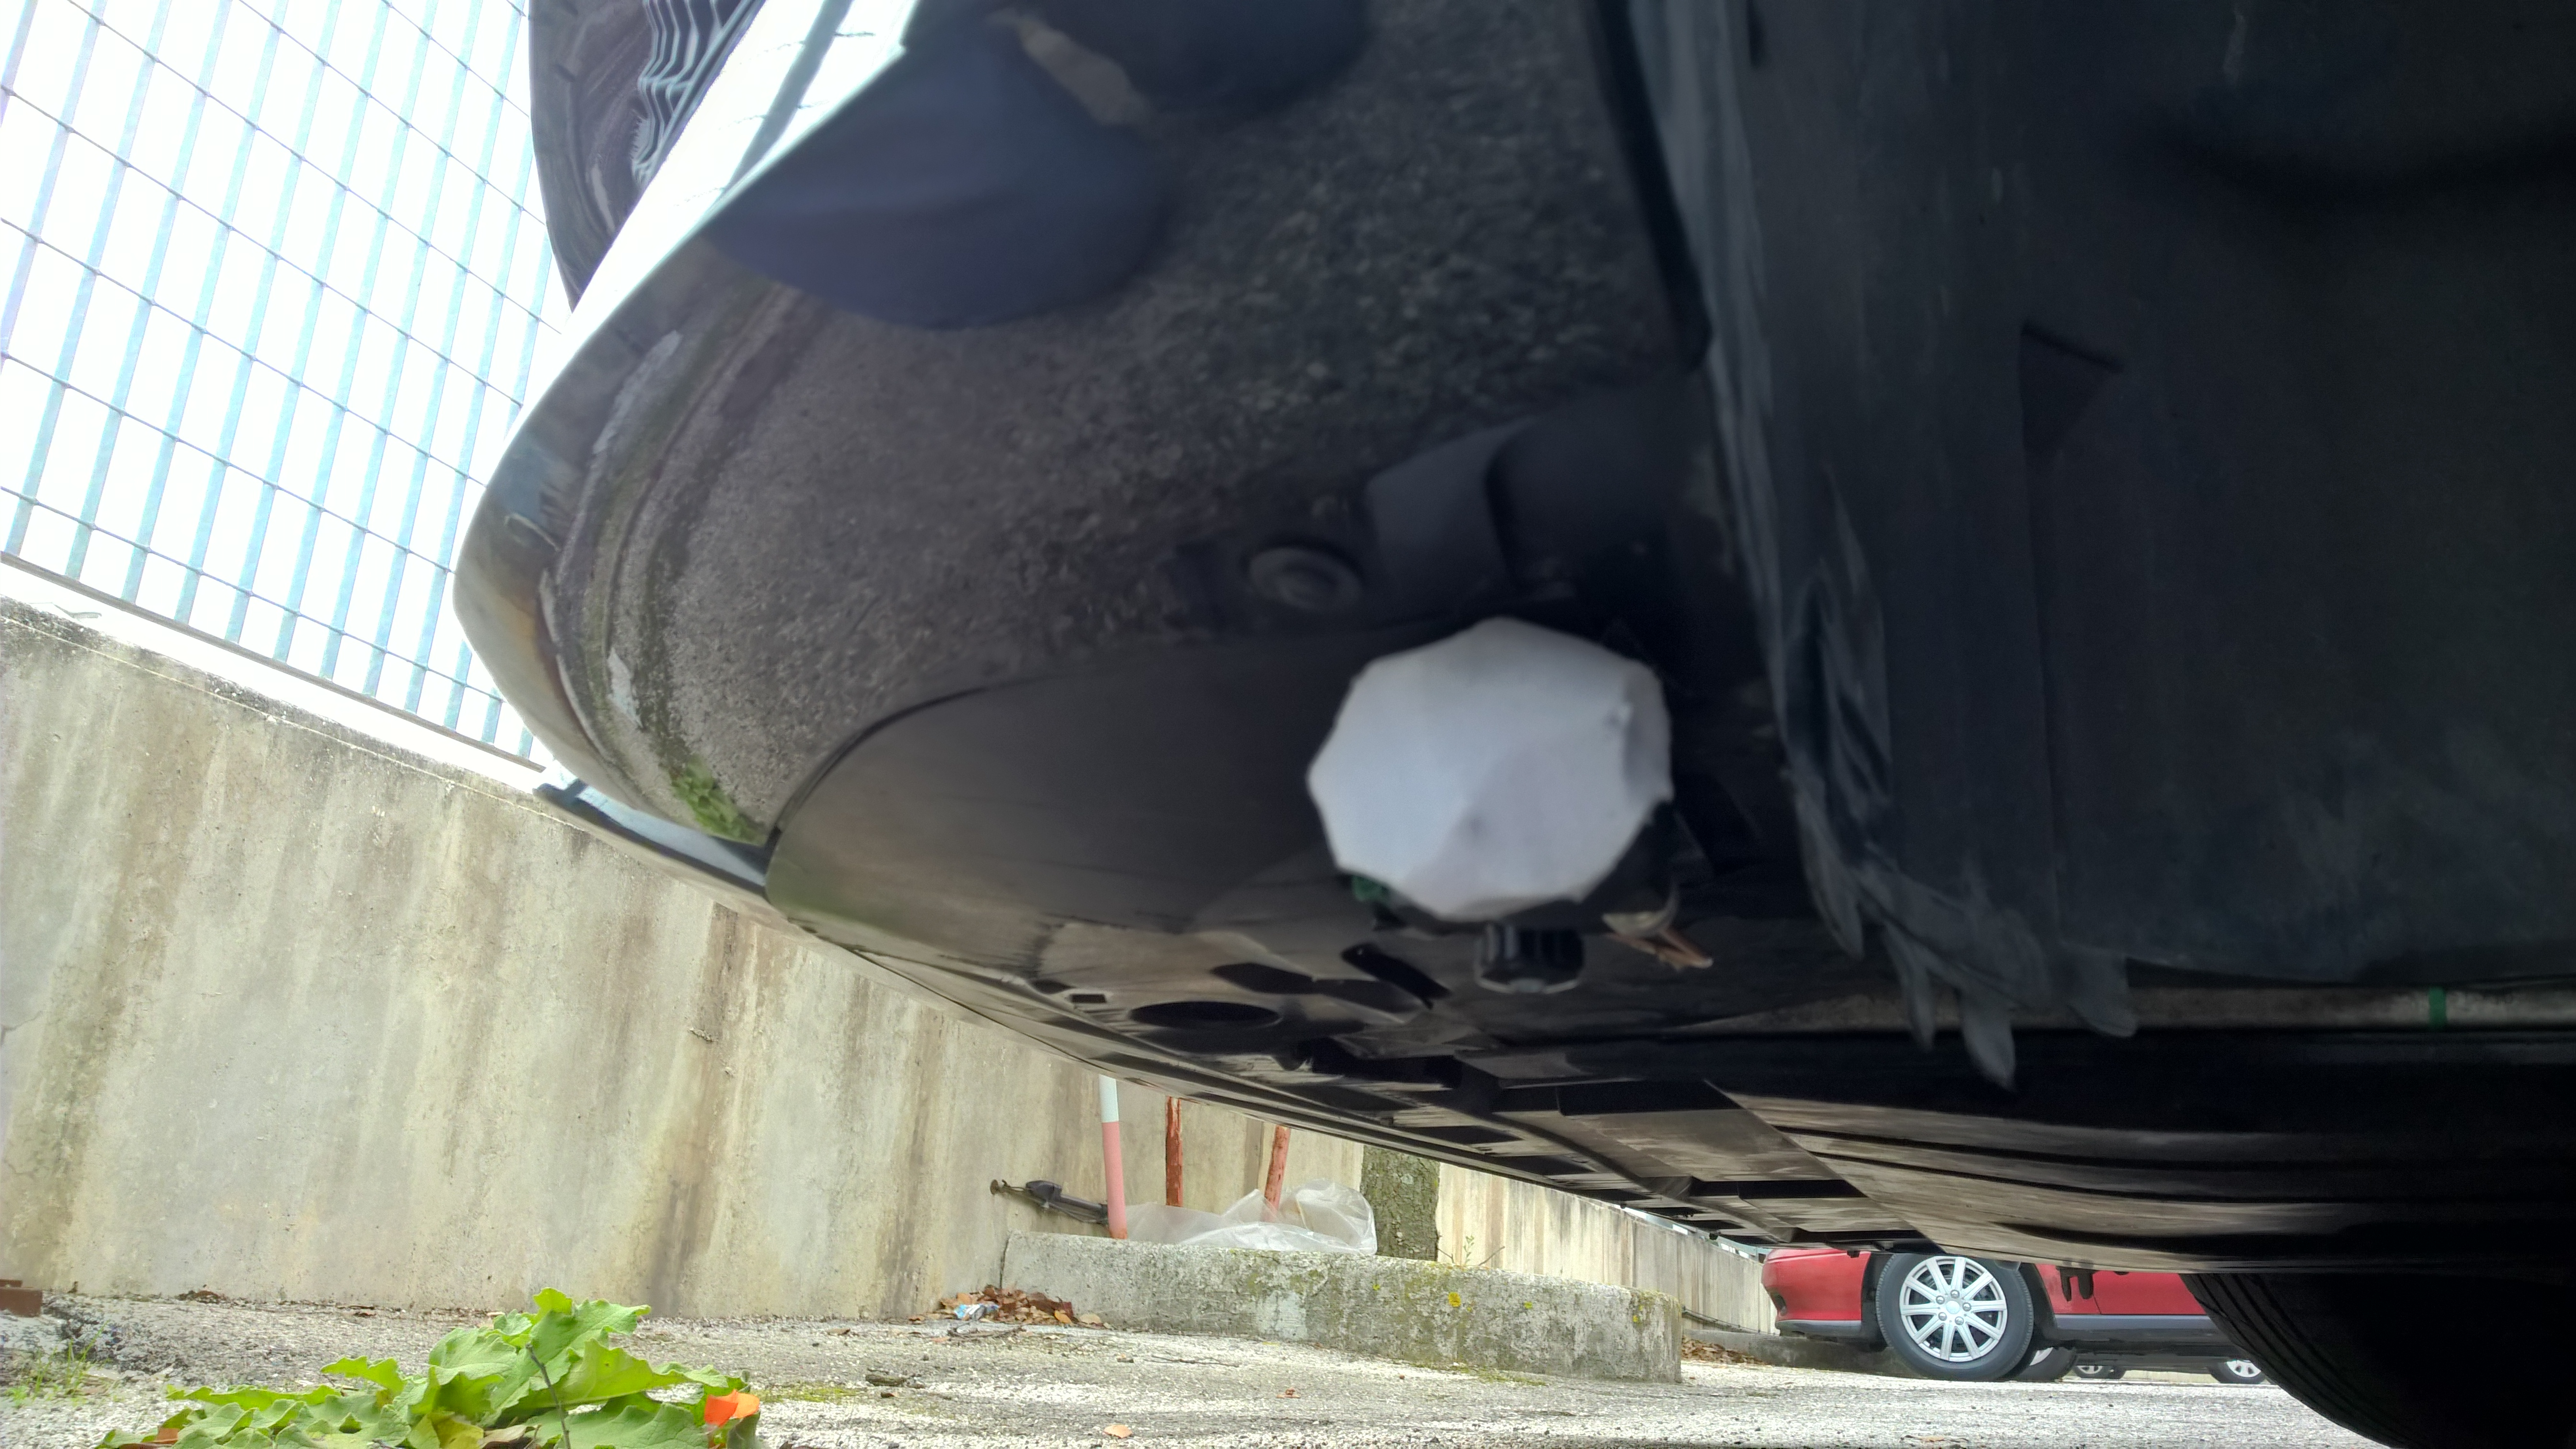
\includegraphics[width=\textwidth]{img/Front-Left.jpg}
		\subcaption{Front left tyre microphone.}
	\end{subfigure}
	
	
	\caption[\textit{PCB Piezotronics} model 130A24 microphones]{Pictures of the \textit{PCB Piezotronics} model 130A24 microphones positioned near the rear right and front left tyres, according to "RR" and "FL" red circles in \figref{fig:car-mic}. The microphones are enclosed by a melamine resin foam with open cell network structure to reduce the wind noise.}
	\label{fig:car-rr-and-fl}
\end{figure}



The car employed to build the dataset is Mercedes A Class from 2014. In addition to the audio signals, the GPS signal has been recorded to track down the car speed and position at any given time. A mobile multi-channel front end, \textit{HEAD Acoustics SQuadriga II}, has been employed as acquisition device, being able to monitor and record 8 contemporary channels at different sample rates, and to store GPS antenna and CAN bus signals.
All audio signals are sampled at 44100\,Hz, 24-bits. The external microphones used -26 dBV as input range while the interior microphones had -16 dBV as input range.
To facilitate the labelling operations, a camcorder \textit{BC Master DC10}\footnote{\url{http://www.bc-master.com/product/car-dash-camera-dc10}} was installed on the dashboard of the car. In addition to the video, it provides the speed information obtained through its own GPS antenna and it records the cockpit audio, useful for taking vocal notes while driving.

The data recorded with the \textit{HEAD Acoustics SQuadriga II} have been exported by means of the software \textit{HEAD Acoustics ArtemiS SUITE} in the uncompressed WAV audio format with a 32-bit float representation.

All recordings were taken in dry conditions in the urban and suburban areas of Ancona (Italy) with variable speed, traffic conditions and pavement roughness. Only roads that had been recently asphalted were considered and multiple takes at different speed for each road have been performed. The dataset is not perfectly balanced and is characterized by 41\% of rough road samples and 59\% of smooth road samples. For this reason a balanced version of the dataset, i.e. with equal number of smooth and rough samples, has been created by pruning excess samples for the most populated class. 
The result of the recording sessions is a 50-minutes-long dataset (41 minutes for the balanced version), with 6 audio channels and a speed channel. Labels for the roads have been annotated manually.

The spectrograms from two audio samples belonging to the smooth and rough classes are shown in Figure \ref{fig:spectrograms_road}.

\begin{figure}[ht]
	\centering
	\begin{subfigure}[b]{0.48\textwidth}
		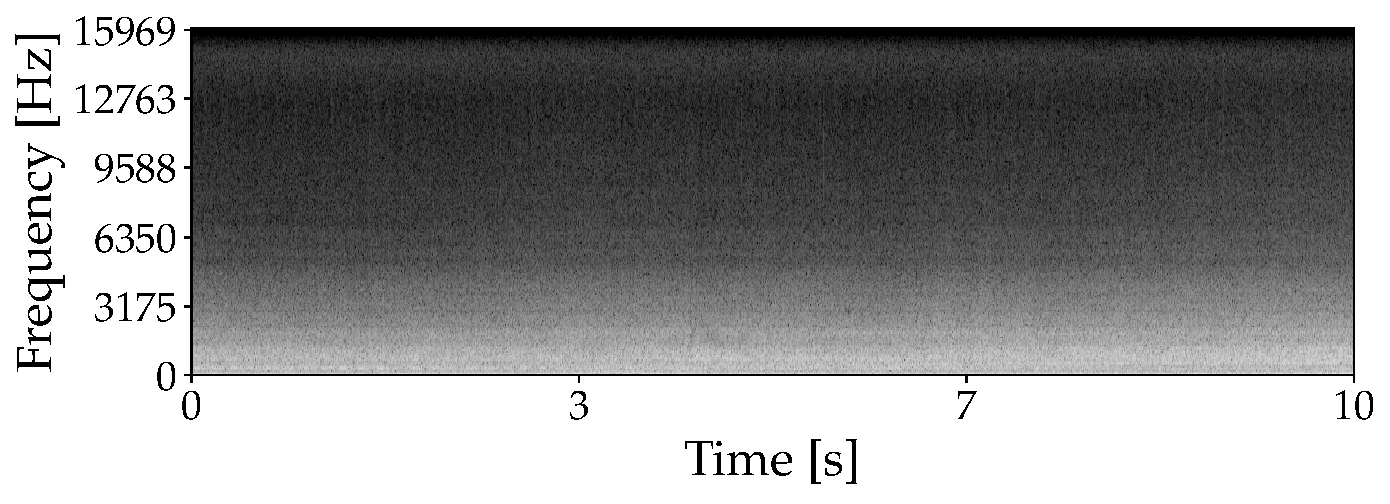
\includegraphics[width=\textwidth]{img/specgram_REC007}
		\subcaption{Smooth road.}
	\end{subfigure}
	\hfil
	\begin{subfigure}[b]{0.48\textwidth}
		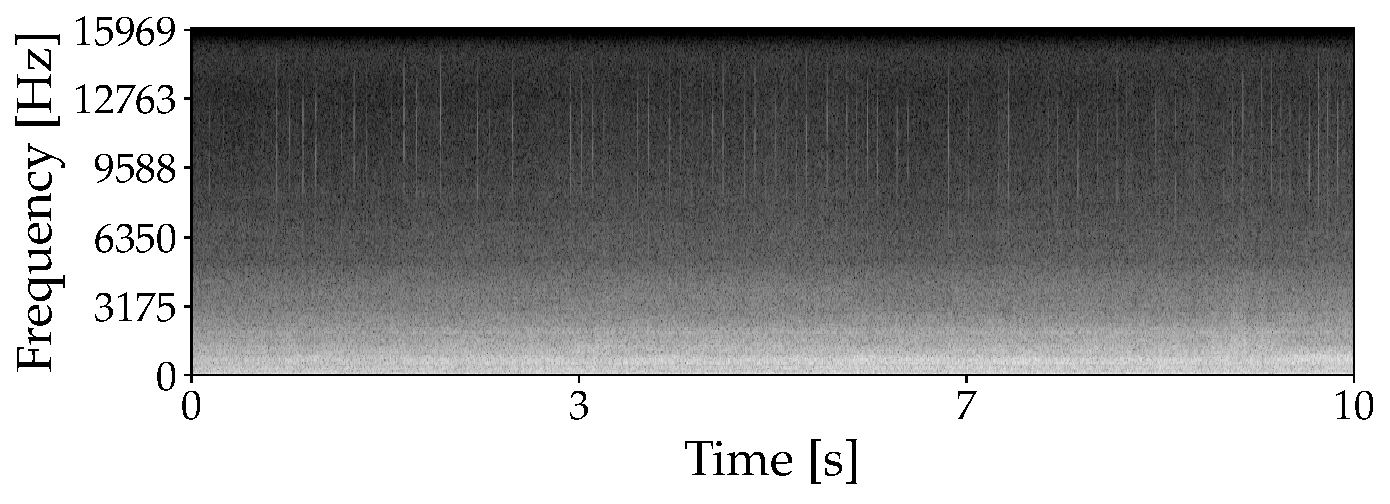
\includegraphics[width=\textwidth]{img/specgram_REC015}
		\subcaption{Rough road.}
	\end{subfigure}
	
	
	\caption[Spectrograms from 10 second samples]{Spectrograms from 10 second samples of (a) smooth urban road, (b) rough highway asphalt.}
	\label{fig:spectrograms_road}
\end{figure}

\subsection{Classification of Snore Sounds Excitation Locations}

\section{The MPSSC dataset}
\label{section:dataset}
The MPSSC dataset is composed of more than 30 hours of audio recordings captured during DISE examinations of 224 subjects from three medical centers recorded between 2006 and 2015. Recording equipment, microphone type, and location differ among the medical centers, so do the background noise characteristics. From the original signals (raw PCM, sample rate 16\,000\,Hz, quantization 16 bit) 843 early identifiable, single site of vibration snore events have been extracted and manually screened from medical experts.
Following the 4-class VOTE scheme, each sound file in the dataset is labelled as V, O, T, E, depending on the tissue from which snore sound originates, as shown in \figref{fig:vote}. They are respectively:
\begin{itemize}
	\item (V) - Velum (palate), including soft palate, uvula, lateral
	velopharyngeal walls;
	\item (O) - Oropharyngeal lateral walls, including palatine tonsils;
	\item (T) - Tongue, including tongue base and airway posterior to the tongue base;
	\item (E) - Epiglottis.
\end{itemize}

\begin{figure}[t]
	\centering
	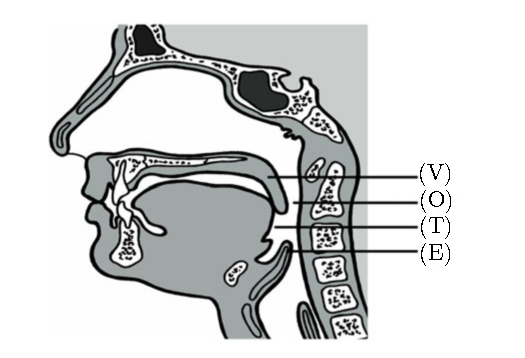
\includegraphics[width=0.6\linewidth]{img/vote.pdf}
	\caption[VOTE positions]{Corresponding positions of the VOTE classification in the upper airway. Picture courtesy of \cite{janott2014akustical}.} 
	\label{fig:vote}
\end{figure}


The dataset is divided into three subsets: \textit{train}, \textit{devel} and \textit{test}.
The number of events per class in the database is strongly unbalanced with a high preeminence of the ``Velum'' (V)-class  and ``Oropharyngeal'' (O)-class (85\% of samples) but in line with the likelihood of occurrence during normal sleep, while 10\% and 5\% of samples respectively belongs to E-events and T-snores. Details of class occurrences are shown in Table I.

\begin{table}[t]
	\centering
	\begin{tabular}{cccc}
		\toprule
		\multicolumn{4}{c}{\textbf{The Munich-Passau Snore Sound Corpus}} \\
		\midrule
		\#  \rule{10pt}{0pt}	& train  \rule{10pt}{0pt} & devel & test\\
		\midrule
		V \rule{10pt}{0pt}	& 168  \rule{15pt}{0pt} & 161 & 155\\
		O \rule{10pt}{0pt}	& 76  \rule{15pt}{0pt} & 75 & 65\\
		T \rule{10pt}{0pt}	& 8  \rule{15pt}{0pt} & 15 & 16\\
		E \rule{10pt}{0pt}	& 30  \rule{15pt}{0pt}& 32 & 27\\
		\bottomrule
		$\Sigma$  \rule{10pt}{0pt} & 282  \rule{13pt}{0pt} & 283 & 263\\
	\end{tabular}
	\caption[The Munich-Passau Snore Sound Corpus]{The Munich-Passau Snore Sound Corpus - The table shows the number of events per class in train, devel and test.}
	\label{tab:mpssc} 
\end{table}

%\begin{figure*}[t]
%	\centering
%	\includegraphics[width=\linewidth]{imgs/spectr-vote.png}
%	\caption{Waveforms and spectrograms of VOTE events}{(a) V (velum); (b) O (oropharyngeal); (c) T (tongue base); (d) E (epiglottis). \textbf{Rifare in HD, eventualmente aggiungere SCAT plot}} 
%	\label{fig:spectrograms}
%\end{figure*}


\begin{figure*}[t]
	\centering
	\begin{subfigure}{.40\textwidth}		
		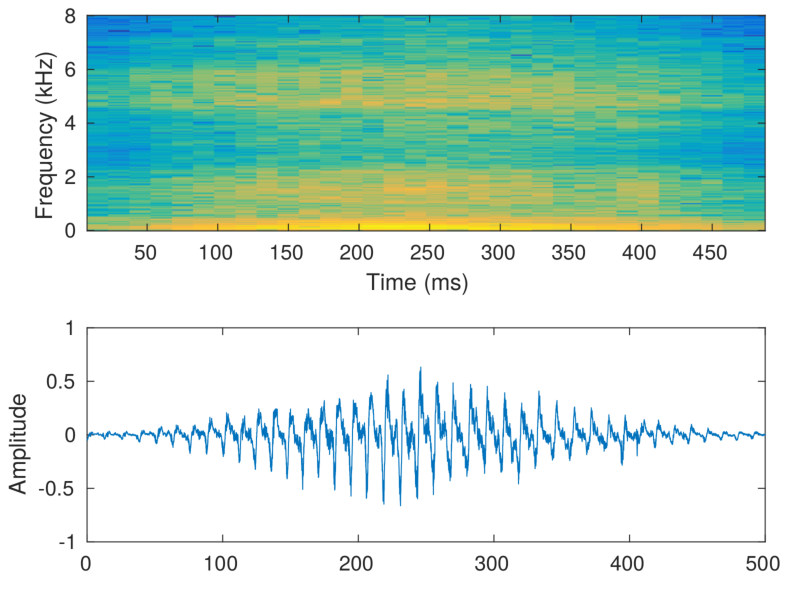
\includegraphics[width=0.9\linewidth]{img/V_spec_crop.pdf}
		\caption{}
		\label{fig:V}
	\end{subfigure}
	\begin{subfigure}{.4\textwidth}
		%\centering
		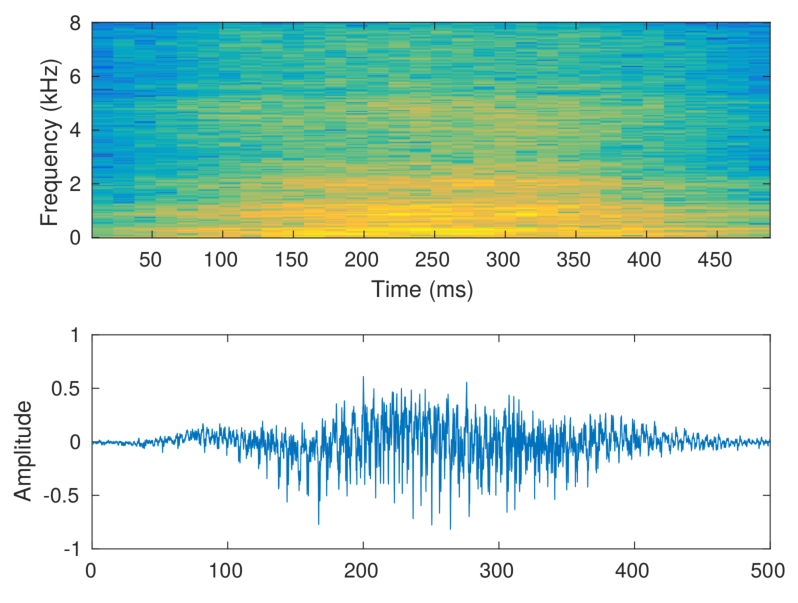
\includegraphics[width=0.9\linewidth]{img/O_spec_crop.pdf}
		\caption{}
		\label{fig:O}
	\end{subfigure}
	\begin{subfigure}{.40\textwidth}
		%\centering
		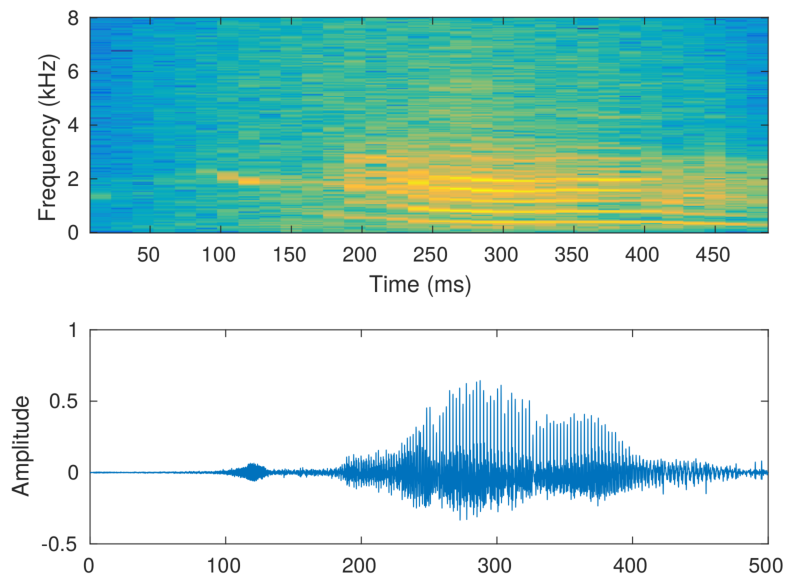
\includegraphics[width=0.9\linewidth]{img/T_spec_crop.pdf}
		\caption{}
		\label{fig:T}
	\end{subfigure}
	\begin{subfigure}{.40\textwidth}
		%\centering
		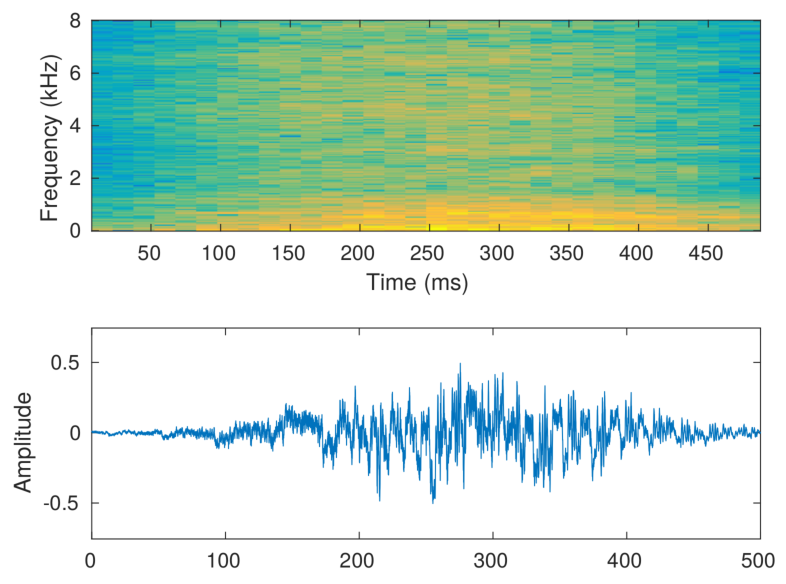
\includegraphics[width=0.9\linewidth]{img/E_spec_crop.pdf}
		\caption{}
		\label{fig:E}
	\end{subfigure}
	\caption{Waveforms and spectrograms of VOTE events}{(a) V (velum); (b) O (oropharyngeal); (c) T (tongue base); (d) E (epiglottis).}
	%\caption{Scat spectrum of VOTE events.  The top image is made of first-order coefficients, organized in a time-scale matrix. at the bottom of the image appear very low frequencies. The second-order coefficients for a fixed scale $m_1$, are shown in the bottom image, again in a time-scale matrix.}{(a) V (velum); (b) O (oropharyngeal); (c) T (tongue base); (d) E (epiglottis).}
	\label{fig:spectrograms}
\end{figure*}
As shown in the waveforms and the related spectrograms in \figref{fig:spectrograms}, the main energy components in three of the classes are concentrated in the frequency area below around 2000 Hz. Energy and spectral distribution characteristics are similar, except for the Type T, which shows higher energy content above 2500 Hz compared to the other three.


\subsection{Bird Audio Detection}
%\label{ssec:dataset}
According to the DCASE 2018 guidelines, the performance of the proposed algorithm has been assessed firstly by using the development dataset for training and validation of the system. Then, a blind test on the provided evaluation dataset was performed with the models which achieved the highest performance and submitted to the organizers of the challenge. The complete dataset is composed of recordings belonging to five different collections. Further details are reported below: %Further details are reported in Table \ref{tab:dataset}.

\begin{itemize}
	\item ``freefield1010'': a collection of 7690 excerpts from field recordings around the world;
	\item ``warblrb10k'': a crowsourced dataset recorded with the \textit{Warblr}\footnote{https://www.warblr.co.uk/} smartphone app. It covers a wide distribution of UK locations and environments and includes weather noise, traffic noise, human speech and even human bird imitations; 8000 samples are used in the development dataset while a held-out set of 2,000 recordings from the same conditions is included in the evaluation split;
	\item ``BirdVox-DCASE-20k'': 20000 files containing remote monitoring flight calls collected from  recordings units placed near Ithaca, NY, USA during the autumn of 2015;
	\item ``Chernobyl'': dataset collected from unattended remote monitoring equipment in the Chernobyl Exclusion Zone (CEZ). A totoal of 6620 audio files cover a range of birds and includes weather, large mammal and insect noise sampled across various CEZ environments, including abandoned village, grassland and forest areas;
	\item ``PolandNFC'': 4000 recordings obtained from a project of monitoring of autumn nocturnal bird migration. They were collected every night, from September to November 2016 on the Baltic Sea coast, Poland, using Song Meter SM2 units with microphones mounted on 3–5 m poles.
\end{itemize}

\begin{table}[t]
	\centering
	\begin{tabular}{|c|c|c|}
		\hline
		\ \textbf{Collection} \rule{0pt}{10pt} & \textbf{N. of samples}  & \textbf{Balance} \\
		\hline
		\hline	
		\multicolumn{3}{|c|}{\textbf{Development Dataset}  \rule{0pt}{10pt}} \\ 
		\hline
		``warblrb10k'' & 8000 & 0.75 \\
		\hline
		``BirdVox-DCASE-20k'' & 20000 & 0.5 \\
		\hline
		``freefield1010'' & 7690 & 0.25 \\
		\hline
		
		Total 	& 35690	& 0.5 \\
		
		\hline
		\hline
		
		\multicolumn{3}{|c|}{\textbf{Evaluation Dataset}  \rule{0pt}{10pt}} \\ 
		\hline
		``warblrb10k\_test'' & 2000 & - \\
		\hline
		``Chernobyl'' & 6620 & - \\
		\hline
		``PolandNFC'' & 4000 & - \\
		\hline
		Total 	& 12620 & - \\
		\hline
	\end{tabular}
	\caption{Details of the dataset we used for the algorithm development. The table shows the number of audio files and the ratio between positive/negative samples (if available) of each used data collection.}
	\label{tab:dataset} 
\end{table}

The organizers recommended a 3-way cross-validation (CV) for the algorithms development, thus in each fold we used two sets for training and the other one as validation set in order to have scores comparable with the others challenge participant.